\documentclass[11pt,a4paper]{article}

\usepackage{fullpage}
\usepackage{hyperref}
\usepackage{graphicx}

\usepackage{caption}
\usepackage{subcaption}
\usepackage{spverbatim}

\usepackage{float}

\usepackage{fancyhdr}
\pagestyle{fancy}
\fancyhf{}
\usepackage{todonotes}                %% notes from the authors

\renewcommand{\headrulewidth}{0pt}
\renewcommand{\footrulewidth}{0pt}

\fancypagestyle{firstpagefooter} {
	\lfoot{\tiny{Version: 25.09.2018}}
	\cfoot{}
	\rfoot{\thepage}
	
}

\lfoot{Name: David Yenicelik Legi: 15-944-366}
\rfoot{\thepage}

\begin{document}

\title{Advanced Systems Lab Report\\ \normalsize{Autumn Semester 2018}}
\author{Name: David Yenicelik \\Legi: 15-944-366}
\date{
	\vspace{4cm}
	\textbf{Grading} \\
	\vspace{0.5cm}
	\begin{tabular}{|c|c|}
		\hline  \textbf{Section} & \textbf{Points} \\
		\hline  1                &                 \\ 
		\hline  2                &                 \\ 
		\hline  3                &                 \\ 
		\hline  4                &                 \\ 
		\hline  5                &                 \\ 
		\hline  6                &                 \\ 
		\hline  7                &                 \\ 
		\hline \hline Total      &                 \\
		\hline 
	\end{tabular} 
}
\maketitle
\thispagestyle{firstpagefooter}

\newpage

\section*{Notes on writing the report \small{(remove this page for submission)}}

Furthermore, it is expected that the interactive law holds for all experiments. In case throughput and response time do not match, it is imperative that you explain why, otherwise you risk losing most of the points for the experiment in question.

\section{System Overview (75 pts)}

I structure my project (code only) into the following folders.
I give a short explanation for each item on how it is used.

I will start out with a diagram that explains the overall structure and refers to each .java file.
I will then be more detailed with my project-code structure.

\begin{figure}[H]
\centering
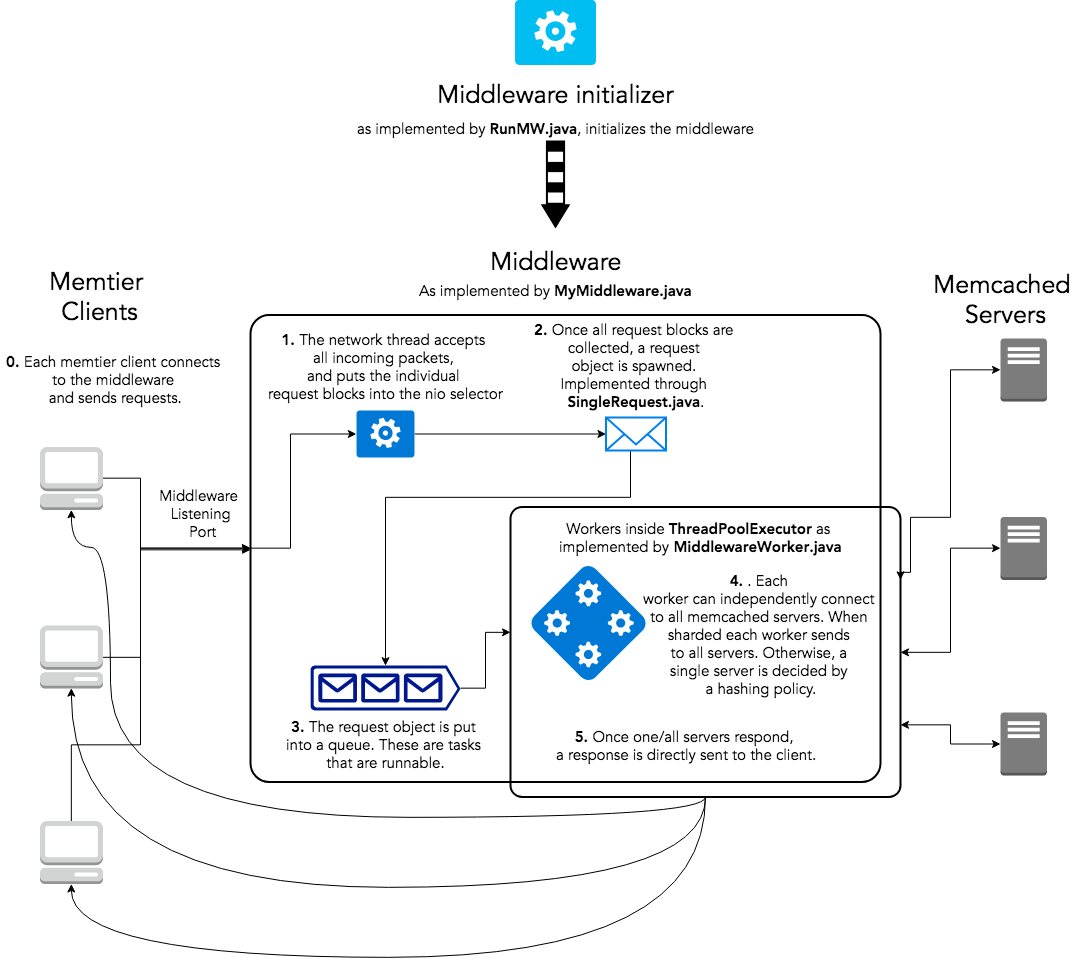
\includegraphics[width=\textwidth]{img/middleware_diagram.png}
\caption{Exp.2.1: A figure with two subfigures}
\label{fig:test}
\end{figure}


\begin{enumerate}
\item \textbf{scripts} \\
This folder includes all the logic to automatically compile the code, deploy the code, run the experiments (each individual one), and automatically download the logs.
This is true both for a local development environment (using docker VM's), and the external "production" environment (using Azure VM's). 
The local docker and external Azure systems are interchangable with a small change in command.

\item \textbf{data} \\
This folder includes all the raw data that is pulled from the experiment, all the python files which process upon this data, and all the processed data.

\item \textbf{figs} \\
This folder includes all the figures that are create using the processed data from point 2.
I use python to create figures from individual graphs

\item \textbf{src} \\
I will talk about the code structure of the src directory with more detail in this next section.
I take a top-down approach while explaining (i.e. starting with where requests originate, and where they go from there).
I will keep this consice, as the \textit{lifetime of a request} section covers some information on what happens in which file.

\begin{enumerate}
\item \textbf{RunMW.java} \\
This is the entry point / main class of the program.
This is the default implementation by the TA's.


\item \textbf{SingleRequest.java} \\
Is the class which encodes a single request from one of the clients.
This can include the SET or GET operation.
For logging purposes, this class also includes all possible times which may be of use to calculate the queueing theory (and latency and throughput) later on.

The request type is parsed by checking the very first character of the request string.
If the string starts with a "g", the request type is a GET (later on, it is decided on the fly if it is a MULTIGET by checking if the number of keys is greater than 1).
If the string starts with a "s", the request type is a SET.
If none of the above cases hold, an error happened (we exit gracefully, as this is unintended behavior).

\item \textbf{MyMiddleware.java} \\
This is the entrypoint of how the Middleware is called.
The datastructure we use to connect to the individual clients is the \textbf{nio.Selector}. 
The \textbf{nio.Selector} can hold multiple connections from different clients conneting. 
Furthermore, it can parse packages that don't immediately fit into the bytebuffer.
The backlog size is bigger than 0 such that multiple requests can made to the same channel at the same time (and these requests are backlogged).


This class is responsible for fetching the individual requests (spawned as a \textit{SingleRequest} object)using non-blocking IO, putting it to a queue, and spawning \textit{MiddlewareWorker}'s within a \textbf{\textit{ThreadPool}} to act upon these requests.
We use the NIO selector to handle all connections.
The entire logic of this .java class runs in on the main thread of the class, which I may refer to as "Network Thread".
This allows for multiple clients to connect to the server in a non-blocking fashion.
Whenever a connection is compelte (i.e. the request is complete), this selector spawns a \textit{MiddlewareWorker} and a \textit{SingleRequest}.

The diagram above symbolizes how this works.

\item \textbf{MiddlewareWorker.java} \\
The \textit{MiddlewareWorker} takes a \textit{SingleRequest} and passes it to the server(s). 
The \textbf{MiddlewareWorker} implements \textbf{Runnable}, and is executed by the \textbf{ThreadPoolExecutor} by calling \textbf{submit}.
Depending on whether the request type is a SET or GET, we have different behavior:

\begin{itemize}
\item case SET: 
The \textit{SingleRequest} is sent to each individual server in a sequential manner.
After the sending to the server is done for all servers, it listens to the response of each individual server.
It listens until all servers have responded.
If any single item has responded with an error, this SET operation responds with the first error encountered to the client.
Otherwise it returns a \textbf{STORED} message. 

\item case GET: 
The string of the \textit{SingleRequest} is used to calculate a hash for the individual request.
This hash is then modulo-ed with the number of server that we can send the request to.
The modulo operation decides which server to send it to.
This has \textbf{provenly uniformly at random distribution}  behavior (proof at: \href{https://eprint.iacr.org/2016/985.pdf, https://en.wikipedia.org/wiki/K-independent_hashing, https://www.akamai.com/es/es/multimedia/documents/technical-publication/consistent-hashing-and-random-trees-distributed-caching-protocols-for-relieving-hot-spots-on-the-world-wide-web-technical-publication.pdf}).
In short, this proof relies on the fact that hashing is pseudorandom, and that pseudorandomity means that for any input, all output values are uniformly at random distributed.
Pseudorandomity keeps it's properties when applied with the modulo operator. 
Because all operations preserve pseudorandomity, the final operation - and thus the server chosen - is also uniformly at random.

\item case MULTIGET (nonsharded):
The nonsharded multiget acts exactly like the GET case.
Again, the uniformly at random assumption is guaranteed because the hashing algorithm is pseudorandom (and as such provides keys uniformly at random).

\item case MULTIGET (sharded):
The sharded MULTIGET case acts as follows. The MULTIGET request is first split up into $n = max(keys, buckets)$ where $buckets$ is the number of servers in total, and $keys$ is the number of keys in total.
Each individual split up request is then treated as an individual GET request.
When the memcached server responds, all the answers are concatenated in a sequential fashion and sent back to the client. 
Errors are handled and also reduced to the first occuring error if this is the case.
\end{itemize}


\item \textbf{LoggerUtils.java} \\
A helper class.
Includes all the logic that is needed to log the requests to hard disk.
All the request logic is accumulated to variables, and the mean is flushed to disk every few minutes.
For GET requests (and in the interest of experiment 5), GET requests are accumulated into a list, and flushed to disk every 5 seconds.
The logging happens in such a way that each individual \textit{MiddlewareWorker} has it's list of requests and all accumulater objects (inside the LoggerUtils.java) to be logged.
Because there is a separate Logger for each thread, there are no issues with multithreading as there is no concurrent data access. \\

Every single request keeps track of the following values, 
which is then flushed to the LoggerUtils.java (and thus to the file)
object when the request has been successfully.
All the information in SingleRequest is used to create the following log-informations.

\begin{enumerate}
\item timeRealOffset
\item differenceTimeCreatedAndEnqueued
\item differenceTimeEnqueuedAndDequeued
\item differenceTimeDequeuedAndSentToServer
\item differenceTimeSentToServerAndReceivedResponseFromServer
\item differenceTimeReceivedResponseFromServerAndSentToClient
\item timeRealDoneOffset
\end{enumerate}

\item \textbf{RequestType.java} \\
A helper struct definition, which defines the two possible input types (Multi-gets are decided on the fly at a different point as described in \textit{SingleRequest.java})

\end{enumerate}

\end{enumerate}

\subsection{Lifetime of a request}
In the following I will talk about how requests enter the middleware, how they are parsed, how they get distributed to servers, and how the middleware communicates these values back to the clients. 
This is a more detailed version of the above diagram.\\

\begin{enumerate}
\item \textbf{Request coming from client to middleware:}\\
When a request comes from a client to the middleware, I use an \textbf{nio.channels.Selector} to accept the request.
This datastructure has the following benefits.
First, it can distinguish between multiple clients.
Second, it can process these individual requests simultaneously in an asynchronous (non-blocking) manner.
Third, it fills up multiple channels (one for each connection, and thus, one for each client), which means that if the request does not fit into one network packet, it will just listen for the rest of the packet.
I detect if a single request fills up by filling a java \textbf{ByteBuffer} until it the request has come to an end (which we can recnognize by waiting for the \textbf{END} keyword.
We parse the type of request by looking at the very first character (interpreting the bytes) and cross-comparing if this is a \textit{set} or \textit{get}. 
To distinguish between \textit{multi-get} and \textit{gets}, we later on split the string resulting from parsing the bytebuffer by spaces.
If the number of elements after splitting is bigger than 2 (the "get" keyword, and the key), then I parse a multi-get.
Else, I parse a get.
\item \textbf{The incoming request spawns a SingleRequest object:}\\
The SingleRequest object is specified in the \textbf{SingleRequest.java} java file and is wrapped around a \textbf{MiddlewareWorker.java} object which implements a java \textbf{Runnable} on which I later on call \textbf{submit} using a \textbf{ThreadPoolExecutor}. 
This file keeps track of the statistics described in the LoggerUtils.java class for logging.
The SingleRequest takes over the \textbf{ByteBuffer} which was created while \textbf{nio.channels.Selector} was listening for a complete network packet.
This ByteBuffer will later on be passed to the individual server(s) (after some processing).
\item \textbf{Submitting a SingleRequest to a MiddlewareWorker using the java ThreadPoolExecutor}:\\
I use the SingleRequest that was generate before, and spawn a new MiddlewareWorker.
This MiddlewareWorker can then be submitted to the java \textbf{ThreadPoolExecutor} which contains the number of middleware-threads (as specified per experiment).
Each individual middlewareworker contains one instantiated \textbf{LoggerUtils} class per thread and thus is threadsafe.
\item \textbf{Sending the server response back to the client}: \\
Each middlewareworker, and thus each individual thread, has a connection to the client that the request came from, and a hashmap of sockets to connect to all the servers.
The response is sent back to the client using the description in the previous sub-section.
In any case, this goes through the individual middleware-worker thread, and does \textbf{not} go through the initial nio.channel.Selector again.
\end{enumerate}

\subsection{Some statistics, and observed bandwidths amongst different VMs}
Some general observations include the following approximate maximum throughput. 
I did not include graphs to this, as all these experiments just involve scalars. \\

I use the program \textit{iperf -c 'VM Address'} to arrive at these statistics.
I arrive at the theoretical maximum throughput by checking how many packages could possibly fit in the bandwidth, where the message size is 4KB, and the bandwidth is specified by the value before that.
I divide the bandwidth by the packet size to arrive at the theoretical maximum throughput per single VM.

\begin{center}
    \begin{tabular}{| l | l | l | l |}
    \hline
    VM From & VM To & Bandwidth & Theoretical Maximum Throughput per VM (ops/sec)\\ \hline
    Client & Middleware & 201 Mbits/sec &  6'250 \\ \hline
    Client & Server & 201 Mbits/sec & 6'250 \\ \hline
    Middleware & Client & 804 Mbits/sec & 25'000 \\ \hline
    Middleware & Server & 804 Mbits/sec & 25'000 \\ \hline
    Server & Client & 101 Mbits/sec &  3'125 \\ \hline
    Server & Middleware & 101 Mbits/sec & 3'125 \\
    \hline
    \end{tabular}
\end{center}

Intuitively, this means that if we have 3 clients and one server, the server must be a bottleneck, and that the clients share the $3'125 ops/s$ (approximately $1'000ops/s$ per client).
\textbf{I will use these numbers to derive some explanations later on}.\\

In addition to the vanilla experiments, I am now talking about my statistical methods of how I analyse the experiments.
Each plotted value for each experiment in the subsequent report was generating using \textbf{three repetitions}, each including a \textbf{warm-up}, and a \textbf{cool-down} phase of 15 seconds (where the core-length of the experiment was 60 seconds.
To arrive at a single rate amongst rates, I use the \textbf{arithmetic mean}.
As an \textbf{error mesaure}, I use the standard deviation.
These are common statistical tools, and according to the \textbf{law of large numbers}, will approximate any distribution truthfully when the number of samples go against infinity, which is why I chose these two measures.

The mean $\mu$ and standard deviation $\sigma$ are calculated as follows:

\begin{equation}
\mu = \frac{\sum_i^n x_i} {n}
\end{equation}

\begin{equation}
\sigma = \sqrt{ \frac{\displaystyle\sum_{i=1}^{n}(x_i - \mu)^2} {n} }
\end{equation}

I will now proceed with the experiments.

\newpage

\section{Baseline without Middleware (75 pts)}
These experiments don't use the middleware, and only consist of memtier client instances, and memcached server instances.

\subsection{One Server}

I use the following setup:

\begin{center}
	\scriptsize{
		\begin{tabular}{|l|c|}
			\hline Number of servers                & 1                        \\ 
			\hline Number of client machines        & 3                        \\ 
			\hline Instances of memtier per machine & 1                        \\ 
			\hline Threads per memtier instance     & 2                        \\
			\hline Virtual clients per thread       & [1..32]                  \\ 
			\hline Workload                         & Write-only and Read-only \\
			\hline Repetitions                      & 3 or more                \\ 
			\hline 
		\end{tabular}
	} 
\end{center}

I will test out the response time and latency for a different number of virtual clients per thread on the client-side (per memtier instance), namely [1, 2, 4, 8, 16, 32].
I will have two different subsections for read-only operations, and write-only operations.
As there is no difference in pre-populating the servers in the case of writes, for both experiments I pre-populate the server the same way as in experiment 2.1 (Baseline without middleware and 3 clients) using the following command, which sequentially generates and stores each key in the server.
\textbf{Wheneverin future experiment setups  I refer to prepopulating the server, I will refer to this command}:

\begin{spverbatim}
      memtier_benchmark -s {SERVER_IP} -p {PORT}
      --protocol=memcache_text --clients={VIRTUAL_CLIENTS_PER_THREAD} --threads={THREADS}
      --requests=15000 --ratio=1:0 --data-size=4096
     --expiry-range=9999-10000 --key-maximum=10000 --key-pattern=S:S
\end{spverbatim}
.\\

The clients and servers don't use multi-gets, and there is no middleware involved.
I run 3 repetitions of each configuration, each having a length of 75 seconds (such that a warm-up and cool-down time of 15 seconds respectively evens out). \\

For the \textbf{read-only experiments}, the throughput reached approximately almost $3000ops/s$, which conforms to the observation of the maximum throughput per server in section 1. 
Please notice that the error is very small, and thus for some points intersects with the measured points.
The error metric (standard deviation) is explained in section 1.\\

For the \textbf{write-only experiments} throughput reached approximately almost $18000ops/s$, which conforms to the observation of the maximum throughput per server in section 1.
Please notice that the error is again very small, and thus barely readable around the measured points. \\

For \textbf{read-only operations}, the bottleneck is the upload bandwidth of the server,
as 3 clients are trying to download a load of 100Mbit/s, and thus must each share appr. 33Mbit/s.
This corresponds to the total upload bandwidth of $3000ops/sec$ (which was empirically proven in section 1 through an additional experiment), is thus divided amongst  three servers.
The missing ops/sec (between our observers ops/sec and $3000$ comes from network overhead.
This also proves to be a valuable sanity check.
The clients are able to generate enough load with even 1 virtual thread per thread, such that with 1 virtual client per thread the network bandwidth is saturated (and stays like this for an increasing number of virtual clients per thread).
As the number of threads increases, more requests are able to be generated.
Because the network bandwidth stays constant, but we introduce more virtual clients, the round-trip time of individual requests increases.
This implies a linear increase in latency, as can be seen from the graph.
This linear increase in the response time provides a second sanity check.

For \textbf{write-only operations}, the bottleneck is the upload bandwidth of the thee clients,
as 3 clients are trying to upload a load of 200Mbit/s each.
The server only responds with message suchs \textit{STORED}, which take up almost no bandwidth compared to the actual message itself.
Thus, the total bandwidth is the additive bandwidth of each individual client, which means approximately $ 3 \times 200 Mbit/s = 600 Mbit/s $, which corresponds to approximately $18000 ops/sec $ (same calculation as in section 1.2). 
The missing ops/sec (between our observers ops/sec and $18000$ comes from network overhead.
This also proves to be a valuable sanity check.
I know that storing the individual requests is not the bottleneck, as a local docker experiment proves that higher throughputs can be achieved locally.
The clients are not able to generate enough load with 1, 2 or 4 virtual clients per thread, and only generate a maximum load with 16 virtual clients per threads, which saturates the upload bandwidth of the client VMs.
This can be seen as the throughput grows square-root like, and then saturates.
This can also be seen from the graph, which plateaus around 16 virtual clients per thread.
As a sanity check, the latency graph shows how the latency does not increase for adding additional virtual clients per thread (although this should increase linearly). 
Only after the 4th virtual client per thread, does the response time increase linearly, which underlines the saturation phase.


\begin{figure}[H]
\centering
\begin{subfigure}{.5\textwidth}
    \centering
    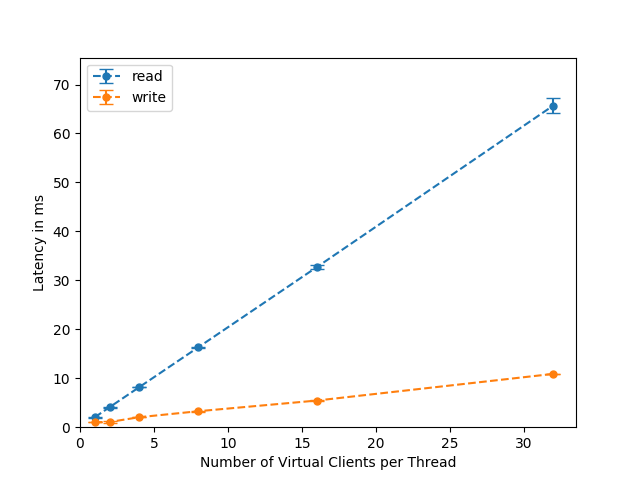
\includegraphics[width=\textwidth]{img/exp2_1/exp2_1__latency_client_read_write.png}
    \caption{Latency write only}
    \label{fig:mesh1}
\end{subfigure}%
\begin{subfigure}{.5\textwidth}
      \centering
    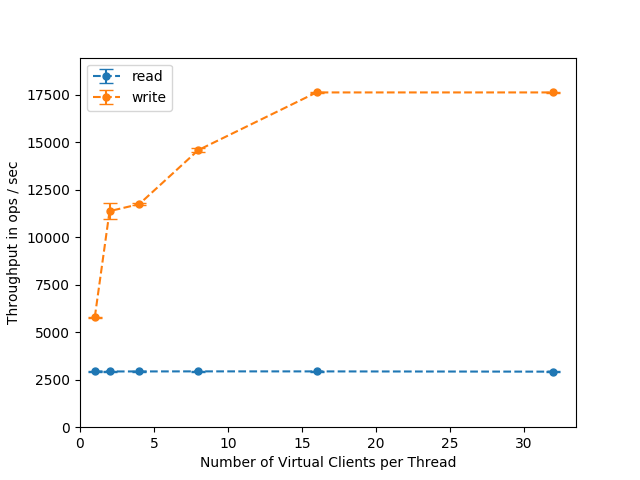
\includegraphics[width=\textwidth]{img/exp2_1/exp2_1__throughput_client_read_write.png}
    \caption{Throughput write only}
    \label{fig:mesh1}
\end{subfigure}
\caption{Exp.2.1: A figure with two subfigures}
\label{fig:test}
\end{figure}

\subsection{Two Servers}

For the following experiment, I use the following setup:

\begin{center}
	\scriptsize{
		\begin{tabular}{|l|c|}
			\hline Number of servers                & 2                        \\ 
			\hline Number of client machines        & 1                        \\ 
			\hline Instances of memtier per machine & 2                        \\ 
			\hline Threads per memtier instance     & 1                        \\
			\hline Virtual clients per thread       & [1..32]                  \\ 
			\hline Workload                         & Write-only and Read-only \\
			\hline Repetitions                      & 3 or more (at least 1 minute each)                \\ 
			\hline 
		\end{tabular}
	} 
\end{center}

I will test out the response time and latency for a different number of virtual clients per thread on the client-side (per memtier instance), namely [1, 2, 4, 8, 16, 32].
As there is no difference in pre-populating the servers in the case of writes, for both experiments I pre-populate the server the same way as in experiment 2.1 (Baseline without middleware and 3 clients).
The clients and servers don't use multi-gets, and there is no middleware involved.
I run 3 repetitions of each configuration, each having a length of 90 seconds (such that the warm-up and cool-down times even out). \\

I first present the graph. 

\begin{figure}[H]
\centering
\begin{subfigure}{.5\textwidth}
    \centering
    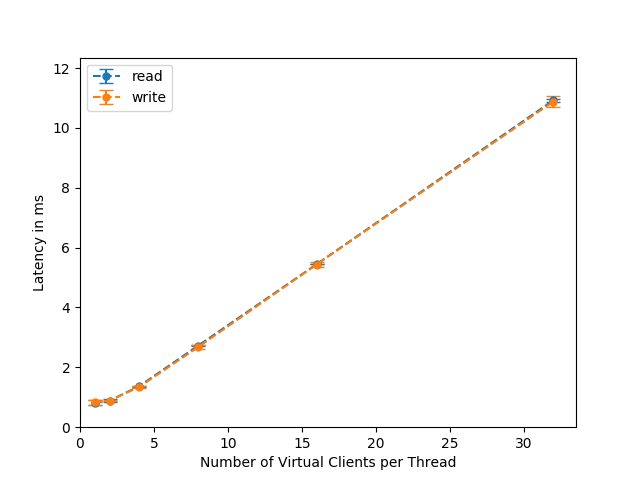
\includegraphics[width=\textwidth]{img/exp2_2/exp2_2__latency_client_read_write.png}
    \caption{Latency write only}
    \label{fig:mesh1}
\end{subfigure}%
\begin{subfigure}{.5\textwidth}
      \centering
    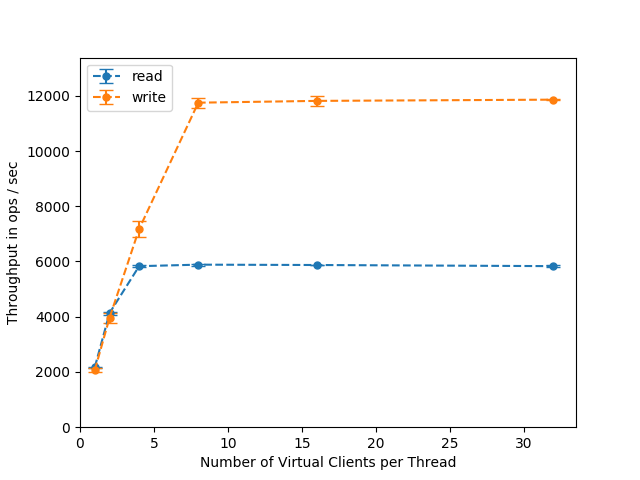
\includegraphics[width=\textwidth]{img/exp2_2/exp2_2__throughput_client_read_write.png}
    \caption{Throughput write only}
    \label{fig:mesh1}
\end{subfigure}
\caption{Exp.2.1: A figure with two subfigures}
\label{fig:test}
\end{figure}

The \textbf{throughput for the read-only experiments} reached approximately almost $6000ops/s$, which conforms to the observation of the maximum throughput per server machine in section 1.
This means that both server virtual machine, are using their maximum capacity to upload all the values that are uploaded by the server virtual machines.
The combined throughput of the two servers is $2 \times 100Mbit/s$ which corresponds to a compound $200Mbit/s$.
This conform to the $6000ops/sec$ when using the same calculation as in section 1.2.

The \textbf{throughput for write-only experiments} reached approximately almost $6000ops/s$, which conforms to the observation of the maximum throughput per client machine in section 1.
This means that both client virtual machines are using their maximum capacity to upload all the values to the server virtual machines.
This conform to the $6000ops/sec$ when using the same calculation as in section 1.2.
Please notice that the error is again very small, and thus intersects with the measured points.
The error metric is explained in section 1.
The server can respond fast enough to all requests by the clients, because the response message (which is usually "STORED") consumes almost none of the bandwidth.\\

Please notice that the error is again very small, and thus intersects with the measured points.
The error metric is explained in section 1. \\

For \textbf{read-only operations}, the bottleneck is the upload bandwidth of the server virtual machines,
as each server is uploading 100Mbit/s each, which compounds to 200Mbit/s together.
The total upload bandwidth of 6000ops/sec (which was empirically proven in section 1 through an additional experiment), is thus divided amongst amongst two memtier servers and thus two memtier instances on the same machine.
This also proves to be a valuable sanity check. \\
The server can respond fast enough to all requests by the clients, as long as there is only up to 4 virtual clients per thread.
Once the client spawns 4 virtual clients per thread, the server VM bandwidth starts to saturate.
The system does not become stable but saturated after an increase of virtual client threads, as can be seen from the plot which indicates that there is no oversaturation.
Because the network bandwidth stays constant, the round-trip time of individual requests increases, except for up to 4 virtual clients per thread.
For 4 virtual clients per threads, the response time stays constant, simply due to the fact that the bandwidth is not saturated, and the requests don't have to wait on each other to be processed (but can be processed in parallel).
This implies an almost constant latency for up to 4 virtual clients per thread, and then an increase in latency, as can be seen from the graph.
The latency and throughput graphs show a correct, inverse correlation.
This almost constant, and linear increase in the response time as seen on the graph provides a second sanity check.


For \textbf{write-only operations}, the bottleneck is the upload bandwidth of the client virtual machines, as the single client is uploading 200Mbit/s each, which compounds to 200Mbit/s together.
Once the client spawns 4 virtual clients per thread, the client VM upload bandwidth starts to saturate as the client upload bandwidth of 200Mbit/s is reached, as each memtier instance in the client is actually able to generate approximately $3'000 ops/sec$, which compounds to $6'000 ops/sec$ when ran on two memtier instances.
The system becomes saturated after an increase of virtual client threads, as can be seen from the plot which indicates that there is minimal to no oversaturation (there is a slight decrease in throughput, but is below some error measures).
Because the network bandwidth stays constant, the round-trip time of individual requests increases, except for up to 4 virtual clients per thread.
For up to 4 virtual clients per threads, the response time grows slowly, simply due to the fact that the bandwidth is not saturated, and the requests don't have to wait on each other to be processed (but can be processed in parallel).
This implies a slow but linear latency for up to 4 virtual clients per thread, and then an increase in latency, as can be seen from the graph.
The latency and throughput graphs show a correct, inverse correlation.
This almost non-steep-linear-trend turns into a and linear increase in the response time as seen on the graph provides a second sanity check. \\

Latency and throughput correlate in the following way. 
The latency is inversely proportional to the throughput.
One can see clearly that this explanation is supported by the two graphs, which show that overall trend of the latency is exponential, while the overall trend of the throughput is logarithmic.
These are inverse functions of each other, as as such provide a sanity check that the experiments go as expected.

\subsection{Summary}

The following table summarizes the quantiative results.

\begin{center}
	{Maximum throughput of different VMs.}
	\begin{tabular}{|l|p{2cm}|p{2cm}|p{4cm}|}
		\hline                        & Read-only workload & Write-only workload & Configuration gives max. throughput \\ 
		\hline One memcached server   & 2940 & 17633 & VC=16  \\ 
		\hline One load generating VM & 5939 & 6054 & VC=8 \\ 
		\hline 
	\end{tabular}
\end{center}

We can compare the read-only and write-only workloads.

The the experiments using \textbf{one memcached server}, the bottleneck is the upload bandwidth of the clients, as was explained in the respective section.
The experiments using \textbf{one load generating VM}, the bottleneck is once the upload bandwidth of the client (for write-only operations), but also the upload bandwidth of the server (for read-only operations). 
A bottleneck occurs exactly if the messages take over the entire network/upload bandwidth, and never happens when only messages such as "GET" or "STORED" are sent back.

For one load generating VM, the read-only and write-only workloads have very similar throughput and latency graphs.
The reason for this is that the upload bandwidth of the compound virtual machines of either clients, or either servers is always capped at $200 Mbit/s$, which implies a maximum throughput of approximately $6'000 ops/sec$.
This conforms to the measurement done in section 1

For one memecached server, this balance is heavily destroyed.
The compound upload bandwidth of the client machines is at approximately $3 \times 200 Mbit/s$, whereas the compound upload bandwidth of the server machines is approximately $100 Mbit/s$.
This means that the clients can send almost any load of operations they want.
However, because the server is capped at $100 Mbit/s$, any read-operations are capped at $3'000 ops/sec$ in total, which can clearly be seen by the graph.
In contrast, write-operations don't suffer this penalty, as the server has almost no bandwidth to give away, as in this case the server only responds with "STORED", and never with a datapacket which is of size $4KB$ (which would fill the bandwidth). 

As such, the configuration with only one memcached server, and the configuration with one load generating VM are in polar contrast to each other, showing that the servers have relatively few bandwidth compared to the client machines, but that the server is fast enough for as long as the bandwidth is not fully used up.

Any numbers that deviate from the theoretical maximum arise due to network overhead, and are statistically insignificant in this analysis.

\section{Baseline with Middleware (90 pts)}

In this set of experiments, I use three client memtier virtual machines, and 1 memcached server.
These virtual machine instances are connected with exactly one middleware virtual machine in the middle.
The three clients connect to the middleware. 
The middleware connects to the server.

The general tendency is that read-only requests are just as fast,
while write-only requests are a bit slower and occur over-saturation in the middleware (probably due to the buffer sizes).

\subsection{One Middleware}

\begin{center}
	\scriptsize{
		\begin{tabular}{|l|c|}
			\hline Number of servers                & 1                        \\ 
			\hline Number of client machines        & 3                        \\ 
			\hline Instances of memtier per machine & 1                        \\ 
			\hline Threads per memtier instance     & 2                        \\
			\hline Virtual clients per thread       & [1..32]                  \\ 
			\hline Workload                         & Write-only and Read-only \\
			\hline Number of middlewares            & 1                        \\
			\hline Worker threads per middleware    & [8..64]                  \\
			\hline Repetitions                      & 3 or more (at least 1 minute each)                \\ 
			\hline 
		\end{tabular}
	} 
\end{center}

The setup is exactly the same as in experiment "Baseline without Middleware and 1 server", with the difference that we inject one middleware between the 
clients, and the server.

In addition the measuring the throughput and response time for different values of number of virtual clients, we also allow to modify the number of middleware threads as another measureable variable.
This means that I test out the throughput and latency for any permutation of
virtualthreads=[1, 2, 4, 8, 16, 32] and threads in the middleware=[8, 16, 32, 64].
I repeat each experiment for 3 times and plot the standard deviation amongst those trials.
I also allow for a 15 second warm-up and 15 second cool-down time, and disregard these measurements when retrieving the logs about the request times from the middleware.\\

The throughput reached approximately almost $3000ops/s$, which conforms to the observation of the maximum throughput per server in section "Baseline without Middleware and 1 server". \\

\subsubsection{Read-only and Explanation}

I will first plot the latency (response time) and the throughput as measured on the middleware.
The throughput reached approximately almost $3000ops/s$, which conforms to the observation of the maximum throughput per server in section 1.
Please notice that the error is again very small, and thus barely readable around the measured points.
The error metric is explained in section 1.
I will later show some plots generated by the logs of the client-machine which underline a correct measurement.

\begin{figure}[H]
\centering
\begin{subfigure}{.5\textwidth}
    \centering
    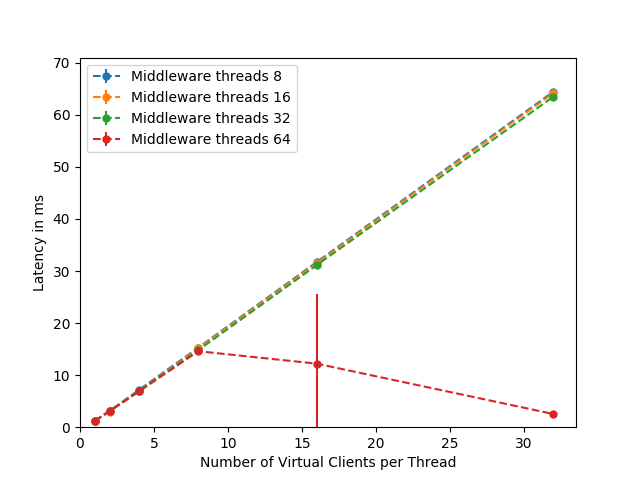
\includegraphics[width=\textwidth]{img/exp3_1/exp3_1__latency_middleware_write_0.png}
    \caption{Exp2.2: Latency read only}
    \label{fig:mesh1}
\end{subfigure}%
\begin{subfigure}{.5\textwidth}
      \centering
    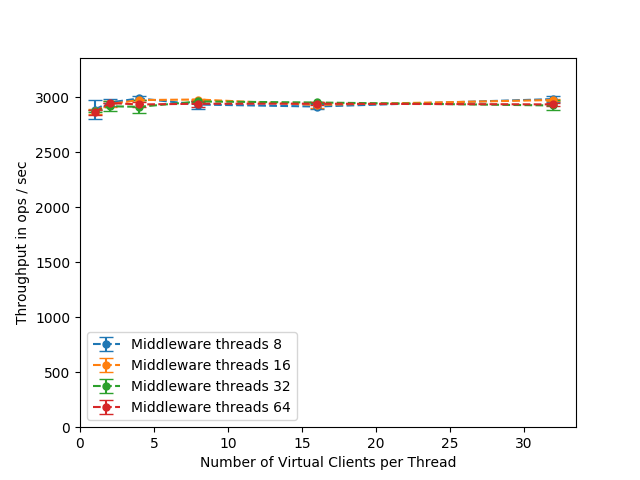
\includegraphics[width=\textwidth]{img/exp3_1/exp3_1__throughput_middleware_write_0.png}
    \caption{Throughput read only}
    \label{fig:mesh1}
\end{subfigure}
\caption{Exp3.1: Latency and throughputs as measures by the \textbf{middlewares}}
\label{fig:test}
\end{figure}

For read-only operations, the bottleneck is the upload bandwidth of the client,
as 3 clients are trying to download a load of 200Mbit/s, and thus must each share appr. 66Mbit/s.
The client is a bottleneck before the middleware, which means that the middleware can easily manage all the read operations from the clients.
The middleware virtual machine does not slow this down, as all GET requests are very short simple requests that all fit into the buffer.
Also, the IO that serves as input to the middleware is non-blocking, which means that it can accept many such small requests simultaneously.
This can be seen as increasing the number of middleware threads does not affect performance, as the client-side is bottlenecked.
Each individual request is sent back to the client through it's designed thread, which does not block the response operation due to a large datasize.
The total upload bandwidth of $3000ops/sec$ (which was empirically proven in section 1 through an additional \textit{iperf} experiment), is thus divided amongst  three clients.
This also proves to be a valuable sanity check.
The difference in the ops/sec (difference between our observers ops/sec and $3'125 ops/sec$ is a reasonable network overhead. 

The clients are able to generate enough load with even 1 virtual client per thread, such that with 1 virtual thread the network bandwidth is saturated.
As the number of threads increases, more requests are able to be generated.
Because the network bandwidth stays constant, the round-trip time of individual requests increases.
This implies an increase in latency.
The linear increase in the latency graph supports this. \\

As a sanity check, I present the throughput and latency plots from the client machines, which all conform to the throughputs and latencies as caluclated in the middleware.
Another sanity check is that the interactive law holds, which states that the response-time \textbf{per request}  is related inversely-linearly proportional to the throughput.

\begin{figure}[H]
\centering
\begin{subfigure}{.5\textwidth}
    \centering
    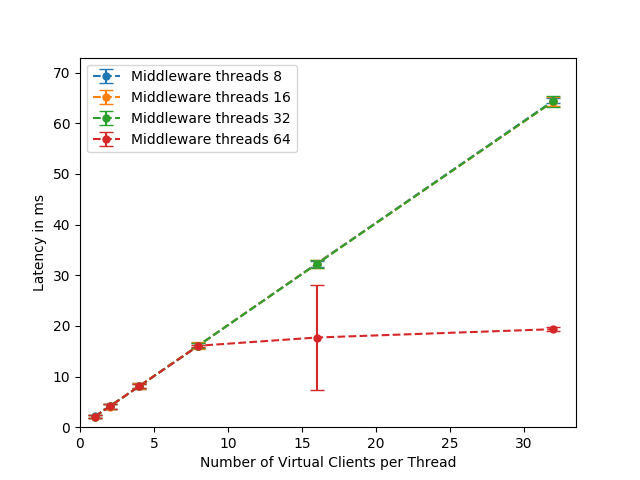
\includegraphics[width=\textwidth]{img/exp3_1/exp3_1__latency_client_write_0.png}
    \caption{Exp2.2: Latency read only}
    \label{fig:mesh1}
\end{subfigure}%
\begin{subfigure}{.5\textwidth}
      \centering
    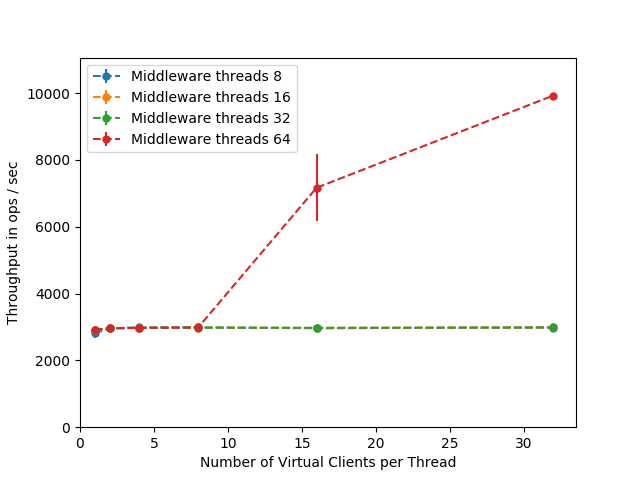
\includegraphics[width=\textwidth]{img/exp3_1/exp3_1__throughput_client_write_0.png}
    \caption{Throughput read only}
    \label{fig:mesh1}
\end{subfigure}
\caption{Exp3.1: Latency and throughputs as measures by the \textbf{clients}}
\label{fig:test}
\end{figure}

The client and middleware graphs deviate sligthly.
As one can see, the middleware graph seems more stable.
This is because the middleware graph only shows the performance \textbf{excluding} the warm-up and cool-down phase (each of which take approximately 15 seconds), whereas the client graphs do not exclude these measurements.

\subsubsection{Write-only and Explanation}

\begin{figure}[H]
\centering
\begin{subfigure}{.5\textwidth}
    \centering
    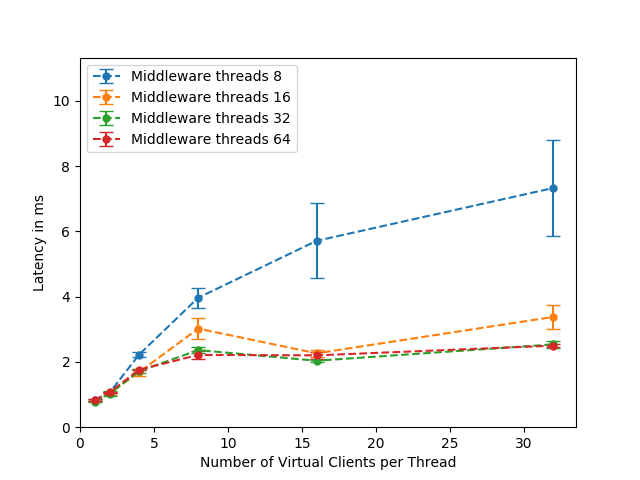
\includegraphics[width=\textwidth]{img/exp3_1/exp3_1__latency_middleware_write_1.png}
    \caption{Latency write only}
    \label{fig:mesh1}
\end{subfigure}%
\begin{subfigure}{.5\textwidth}
      \centering
    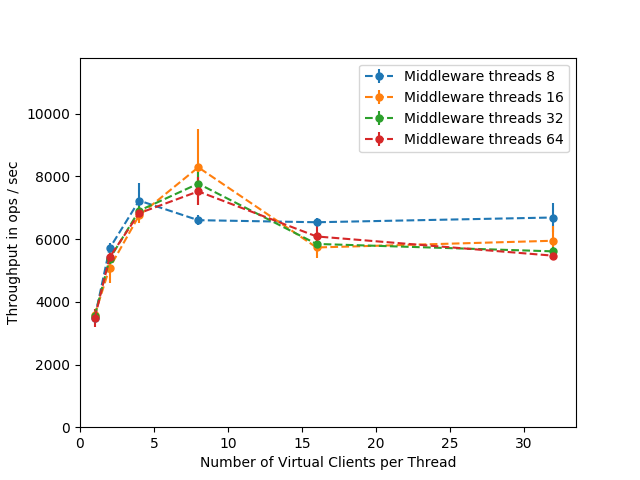
\includegraphics[width=\textwidth]{img/exp3_1/exp3_1__throughput_middleware_write_1.png}
    \caption{Throughput write only}
    \label{fig:mesh1}
\end{subfigure}
\caption{Exp3.1: Latency and throughputs as measures by the middlewares}
\label{fig:test}
\end{figure}

The single server is fast enough to respond to all individual client requests, as the server is only responding with the message "STORED" each time.
However, at some point, the number of requests is so high, that either the individual client output bandwidth, or storing the actual requests on the hard-ware side becomes the bottleneck.
This can be seen as the throughput grows square-root like, and then saturates.
The throughput graph, which means out with 16 virtual clients per thread, proves this point.
To decide whether the network is the bandwidth is the bottleneck, I repeat this experiment locally with virtual docker containers.
These plateau at a later stage, which proves that the maximum network bandwidth is reached with 16 virtual clients per thread.

%TODO :
Latency and throughput correlate in the following way: \textbf{???}

The following graphs are created using the logs of the client for the throughput and the latency, and underline that the values are sane.

As a sanity check, I present the throughput and latency plots from the client machines, which all conform to the throughputs and latencies as caluclated in the middleware.
Another sanity check is that the interactive law holds, which states that the response-time \textbf{per request}  is related inversely-linearly proportional to the throughput.

\begin{figure}[H]
\centering
\begin{subfigure}{.5\textwidth}
    \centering
    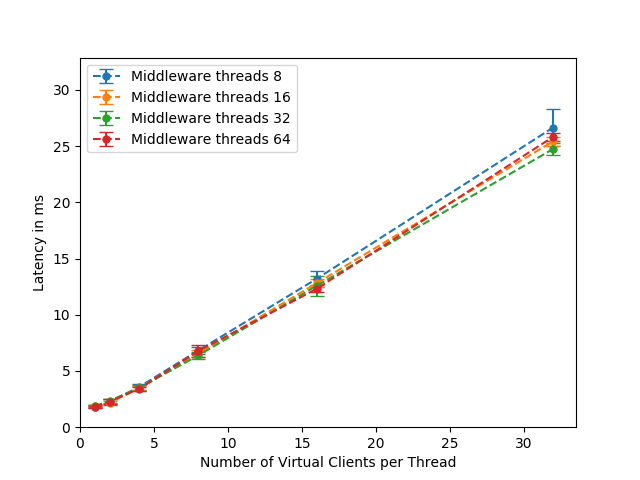
\includegraphics[width=\textwidth]{img/exp3_1/exp3_1__latency_client_write_1.png}
    \caption{Latency write only}
    \label{fig:mesh1}
\end{subfigure}%
\begin{subfigure}{.5\textwidth}
      \centering
    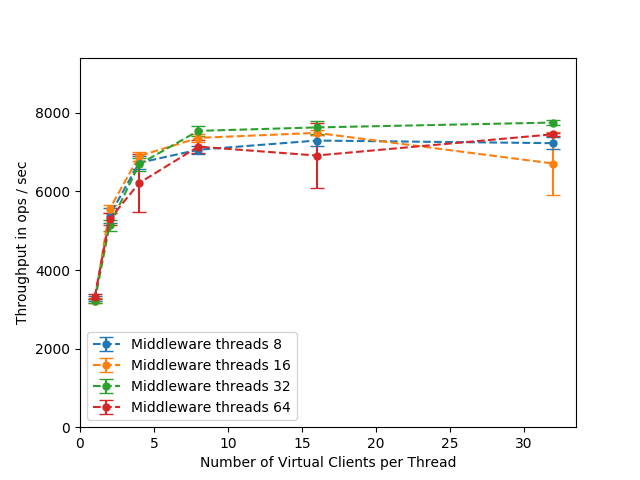
\includegraphics[width=\textwidth]{img/exp3_1/exp3_1__throughput_client_write_1.png}
    \caption{Throughput write only}
    \label{fig:mesh1}
\end{subfigure}
\caption{Exp3.1: Latency and throughputs as measures by the clients}
\label{fig:test}
\end{figure}




The client and middleware graphs deviate sligthly.
As one can see, the middleware graph seems more stable.
This is because the middleware graph only shows the performance \textbf{excluding} the warm-up and cool-down phase, whereas the client graphs do not exclude these measurements.

\subsubsection{Additional Explanation}

%TODO : compare read-only and write-only operations 

Provide a detailed analysis of the results (e.g., bottleneck analysis, component utilizations, average queue lengths, system saturation). Add any additional figures and experiments that help you illustrate your point and support your claims.

\subsection{Two Middlewares}

\begin{center}
	\scriptsize{
		\begin{tabular}{|l|c|}
			\hline Number of servers                & 1                        \\ 
			\hline Number of client machines        & 3                        \\ 
			\hline Instances of memtier per machine & 2                        \\ 
			\hline Threads per memtier instance     & 1                        \\
			\hline Virtual clients per thread       & [1..32]                  \\ 
			\hline Workload                         & Write-only and Read-only \\
			\hline Number of middlewares            & 2                        \\
			\hline Worker threads per middleware    & [8..64]                  \\
			\hline Repetitions                      & 3 or more (at least 1 minute each)                \\ 
			\hline 
		\end{tabular}
	} 
\end{center}

The setup is exactly the same as in experiment "Baseline without Middleware and 1 server", with the difference that we inject two middlewares between the clients, and the server.
Another difference is that we allow each individual client to run two memtier instances (each with one thread) to be able to connect to two instances each.
The throughput reached approximately almost $3000ops/s$, which conforms to the observation of the maximum throughput per server in section "Baseline without Middleware and 1 server". \\

In addition the measuring the throughput and response time for different values of number of virtual clients, we also allow to modify the number of middleware threads as another measureable variable.
This means that I test out the throughput and latency for any permutation of
virtualthreads=[1, 2, 4, 8, 16, 32] and threads in the middleware=[8, 16, 32, 64].
I repeat each experiment for 3 times and plot the standard deviation amongst those trials.
I also allow for a 15 second warm-up and 15 second cool-down time, and disregard these measurements when retrieving the logs about the request times from the middleware.\\

Connect three load generator machines (two instances of memtier with CT=1) to two middlewares and use 1 memcached server. Run a read-only and a write-only workload with increasing number of clients (between 2 and 64) and measure response time \emph{both at the client and at the middleware}, and plot the throughput and response time as measured in the middleware.

Repeat this experiment for different number of worker threads inside the middleware: 8, 16, 32, 64.

\begin{center}
	\scriptsize{
		\begin{tabular}{|l|c|}
			\hline Number of servers                & 1                        \\ 
			\hline Number of client machines        & 3                        \\ 
			\hline Instances of memtier per machine & 2                        \\ 
			\hline Threads per memtier instance     & 1                        \\
			\hline Virtual clients per thread       & [1..32]                  \\ 
			\hline Workload                         & Write-only and Read-only \\
			\hline Multi-Get behavior               & N/A                      \\
			\hline Multi-Get size                   & N/A                      \\
			\hline Number of middlewares            & 2                        \\
			\hline Worker threads per middleware    & [8..64]                  \\
			\hline Repetitions                      & 3 or more (at least 1 minute each)                \\ 
			\hline 
		\end{tabular}
	} 
\end{center}

\subsubsection{Read-only}

\begin{figure}[H]
\centering
\begin{subfigure}{.5\textwidth}
    \centering
    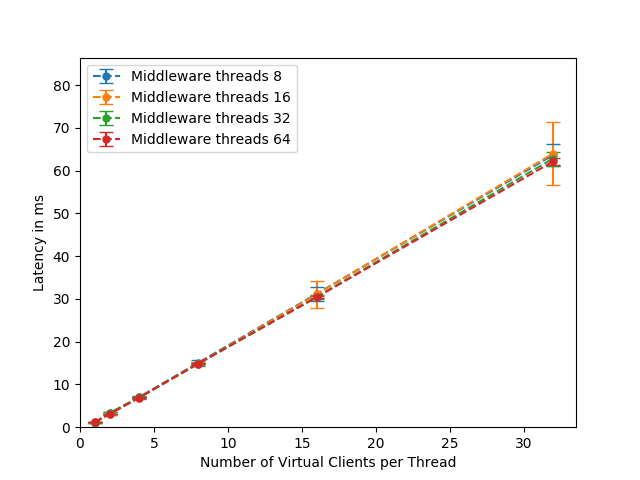
\includegraphics[width=\textwidth]{img/exp3_2/exp3_2__latency_middleware_write_0.png}
    \caption{Latency read only}
    \label{fig:mesh1}
\end{subfigure}%
\begin{subfigure}{.5\textwidth}
      \centering
    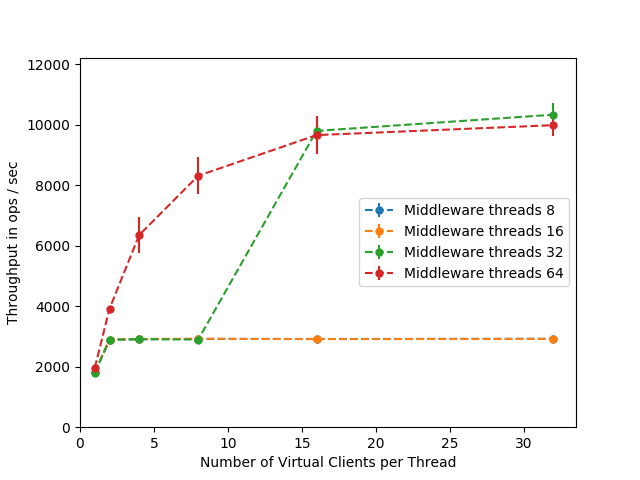
\includegraphics[width=\textwidth]{img/exp3_2/exp3_2__throughput_middleware_write_0.png}
    \caption{Throughput read only}
    \label{fig:mesh1}
\end{subfigure}
\caption{Exp3.2: Latency and throughputs as measures by the middlewares}
\label{fig:test}
\end{figure}

%TODO : explanation

\begin{figure}[H]
\centering
\begin{subfigure}{.5\textwidth}
    \centering
    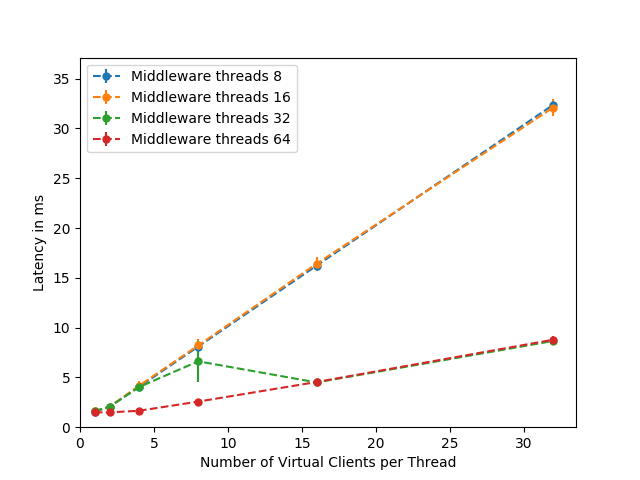
\includegraphics[width=\textwidth]{img/exp3_2/exp3_2__latency_client_write_0.png}
    \caption{Latency read only}
    \label{fig:mesh1}
\end{subfigure}%
\begin{subfigure}{.5\textwidth}
      \centering
    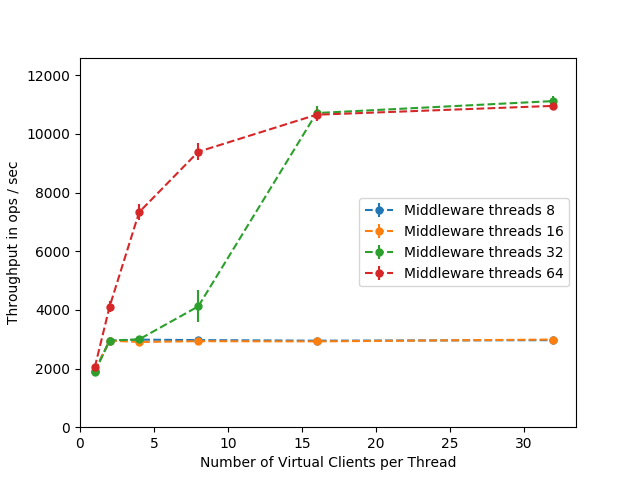
\includegraphics[width=\textwidth]{img/exp3_2/exp3_2__throughput_client_write_0.png}
    \caption{Throughput read only}
    \label{fig:mesh1}
\end{subfigure}
\caption{Exp3.2: Latency and throughputs as measures by the clients}
\label{fig:test}
\end{figure}

The client and middleware graphs deviate sligthly.
As one can see, the middleware graph seems more stable.
This is because the middleware graph only shows the performance \textbf{excluding} the warm-up and cool-down phase, whereas the client graphs do not exclude these measurements.


\subsubsection{Write-only}

\begin{figure}[H]
\centering
\begin{subfigure}{.5\textwidth}
    \centering
    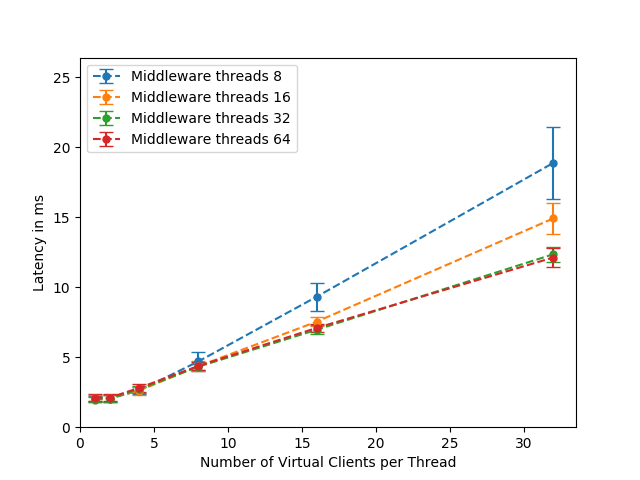
\includegraphics[width=\textwidth]{img/exp3_2/exp3_2__latency_client_write_1.png}
    \caption{Latency write only}
    \label{fig:mesh1}
\end{subfigure}%
\begin{subfigure}{.5\textwidth}
      \centering
    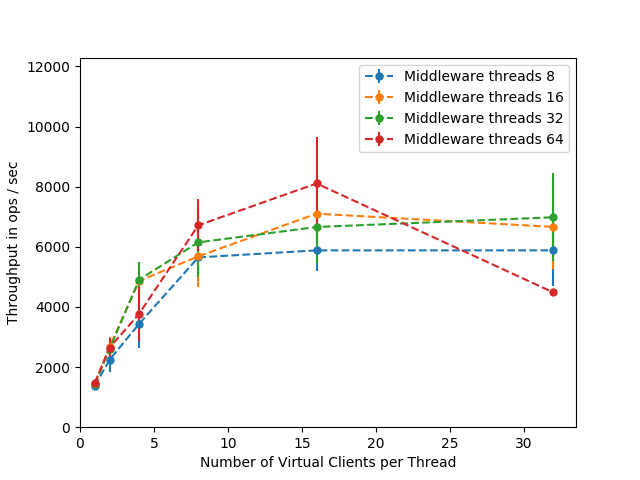
\includegraphics[width=\textwidth]{img/exp3_2/exp3_2__throughput_client_write_1.png}
    \caption{Throughput write only}
    \label{fig:mesh1}
\end{subfigure}
\caption{Exp3.2: Latency and throughputs as measures by the clients}
\label{fig:test}
\end{figure}

%TODO : explanation

\begin{figure}[H]
\centering
\begin{subfigure}{.5\textwidth}
    \centering
    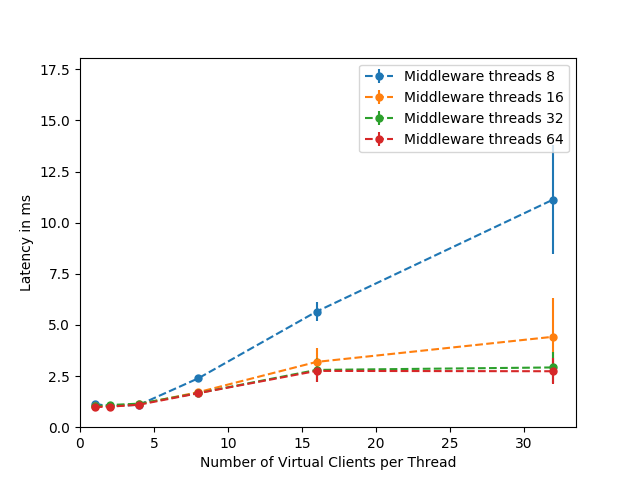
\includegraphics[width=\textwidth]{img/exp3_2/exp3_2__latency_middleware_write_1.png}
    \caption{Latency write only}
    \label{fig:mesh1}
\end{subfigure}%
\begin{subfigure}{.5\textwidth}
      \centering
    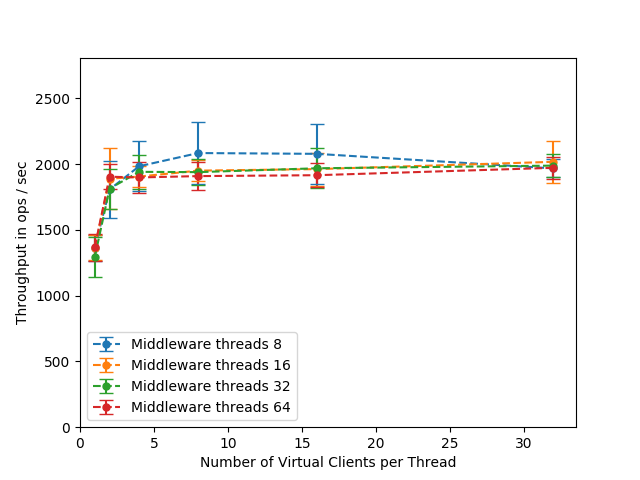
\includegraphics[width=\textwidth]{img/exp3_2/exp3_2__throughput_middleware_write_1.png}
    \caption{Throughput write only}
    \label{fig:mesh1}
\end{subfigure}
\caption{Exp3.2: Latency and throughputs as measures by the middlewares}
\label{fig:test}
\end{figure}

The client and middleware graphs deviate sligthly.
As one can see, the middleware graph seems more stable.
This is because the middleware graph only shows the performance \textbf{excluding} the warm-up and cool-down phase, whereas the client graphs do not exclude these measurements.

\subsubsection{Explanation}

Provide a detailed analysis of the results (e.g., bottleneck analysis, component utilizations, average queue lengths, system saturation). Add any additional figures and experiments that help you illustrate your point and support your claims.

\subsection{Summary}

Based on the experiments above, fill out the following table. For both of them use the numbers from a single experiment to fill out all lines. Miss rate represents the percentage of GET requests that return no data. Time in the queue refers to the time spent in the queue between the net-thread and the worker threads.


\begin{center}
	{Maximum throughput for one middleware.}
	\begin{tabular}{|l|p{2cm}|p{2cm}|p{2cm}|p{2cm}|}
		\hline                                & Throughput & Response time & Average time in queue & Miss rate \\ 
		\hline Reads: Measured on middleware  & 2933 & 64 &                       &           0 \\ 
		\hline Reads: Measured on clients     & 2987 & 64 & n/a                   &           0 \\ 
		\hline Writes: Measured on middleware & 8291 & 7 &                       & n/a       \\ 
		\hline Writes: Measured on clients    & 7423 & 34 & n/a                   & n/a       \\ 
		\hline 
	\end{tabular}
\end{center}

\begin{center}
	{Maximum throughput for two middlewares.}
	\begin{tabular}{|l|p{2cm}|p{2cm}|p{2cm}|p{2cm}|}
		\hline                                & Throughput & Response time & Average time in queue & Miss rate \\ 
		\hline Reads: Measured on middleware  & 10330 & 31.40 &                       &           0\\ 
		\hline Reads: Measured on clients     & 11116 &  32.37 & n/a                   &           0\\ 
		\hline Writes: Measured on middleware & 8131 & 11.13 &                       & n/a       \\ 
		\hline Writes: Measured on clients    & 8108 & 14.27 & n/a                   & n/a       \\ 
		\hline 
	\end{tabular}
\end{center}

Notice that the miss rate is always zero, because this is 1. a closed system, and all servers are pre-populated before any experiment starts.

Based on the data provided in these tables, write at least two paragraphs summarizing your findings about the performance of the middleware in the baseline experiments.

\section{Throughput for Writes (90 pts)}

\subsection{Full System}
I am connecting three load generating client VMs to two middlewares.
These middlewares are connected to three memcached server VMs each.
I have the following setup.

\begin{center}
	\scriptsize{
		\begin{tabular}{|l|c|}
			\hline Number of servers                & 3          \\ 
			\hline Number of client machines        & 3          \\ 
			\hline Instances of memtier per machine & 2          \\ 
			\hline Threads per memtier instance     & 1          \\
			\hline Virtual clients per thread       & [1..32]    \\ 
			\hline Workload                         & Write-only \\
			\hline Number of middlewares            & 2          \\
			\hline Worker threads per middleware    & [8..64]    \\
			\hline Repetitions                      & 3 or more (at least 1 minute each)  \\ 
			\hline 
		\end{tabular}
	} 
\end{center}

During this experiment, I iterate over all possible permutations of virtual clients per thread (in the range of [1, 2, 4, 8, 16, 32]), and worker threads per middlewares (in the range of [8, 16, 32, 64]).
I run each experiment for 90 seconds (which includes a 15 second warm-up and a 15 second cool-down time). 
Each experiment again consists of three trials from which we measure the mean and the standard deviation.
This section only covers write-only experiments.
I cover response time (latency) , and throughput. \\

The following are graphs from the middleware.

\begin{figure}[H]
\centering
\begin{subfigure}{.5\textwidth}
    \centering
    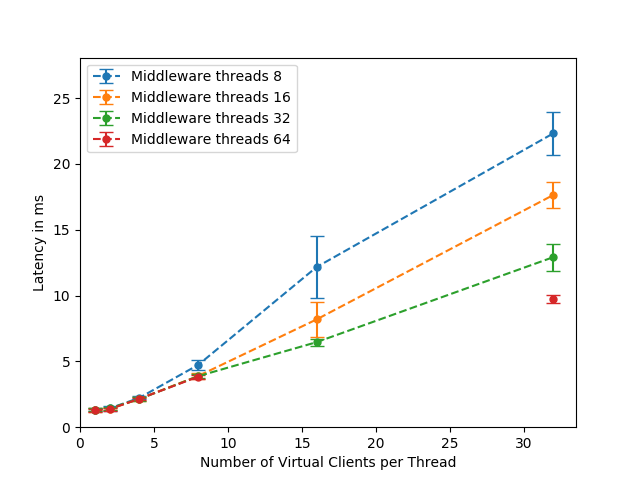
\includegraphics[width=\textwidth]{img/exp4_1/exp4_1__vc_64__latency_middleware_write_1.png}
    \caption{Latency write only}
    \label{fig:mesh1}
\end{subfigure}%
\begin{subfigure}{.5\textwidth}
      \centering
    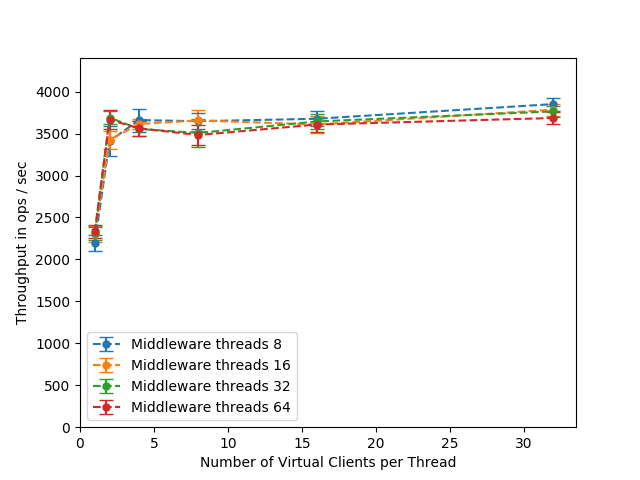
\includegraphics[width=\textwidth]{img/exp4_1/exp4_1__vc_64__throughput_middleware_write_1.png}
    \caption{Throughput write only}
    \label{fig:mesh1}
\end{subfigure}
\caption{Exp3.2: Latency and throughputs as measures by the middlewares}
\label{fig:test}
\end{figure}

\begin{figure}[H]
\centering
\begin{subfigure}{.5\textwidth}
    \centering
    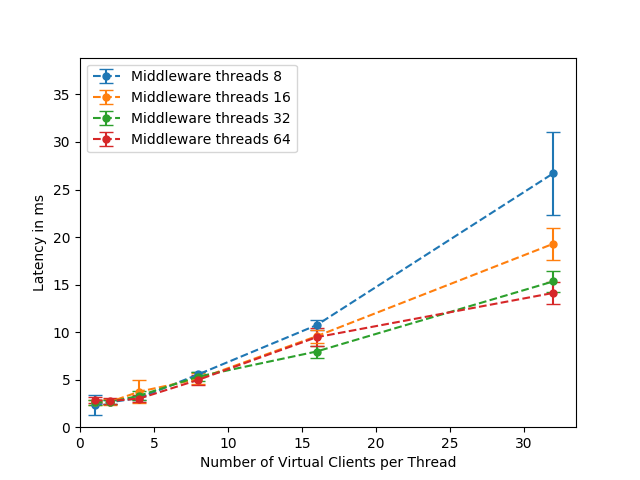
\includegraphics[width=\textwidth]{img/exp4_1/exp4_1__vc_64__latency_client_write_1.png}
    \caption{Latency write only}
    \label{fig:mesh1}
\end{subfigure}%
\begin{subfigure}{.5\textwidth}
      \centering
    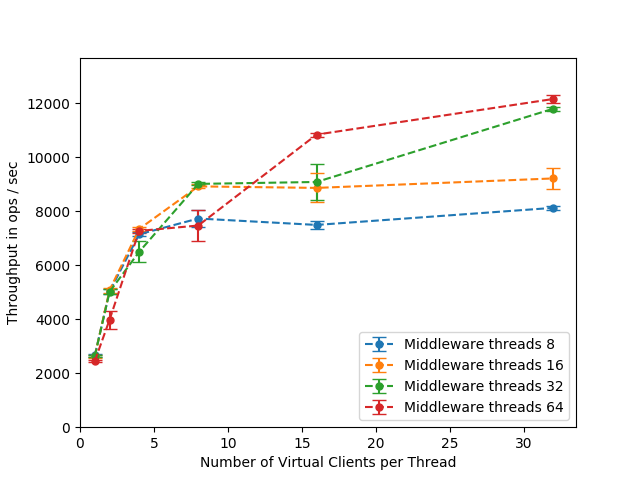
\includegraphics[width=\textwidth]{img/exp4_1/exp4_1__vc_64__throughput_client_write_1.png}
    \caption{Throughput write only}
    \label{fig:mesh1}
\end{subfigure}
\caption{Exp3.2: Latency and throughputs as measures by the clients}
\label{fig:test}
\end{figure}

\subsubsection{Explanation}

Provide a detailed analysis of the results (e.g., bottleneck analysis, component utilizations, average queue lengths, system saturation). Add any additional figures and experiments that help you illustrate your point and support your claims.

\subsection{Summary}

Based on the experiments above, fill out the following table with the data corresponding to the maximum throughput point for all four worker-thread scenarios.

\begin{center}
	{Maximum throughput for the full system}
	\begin{tabular}{|l|p{1.5cm}|p{1.5cm}|p{1.5cm}|p{1.5cm}|}
		\hline                                            & WT=8 & WT=16 & WT=32 & WT=64 \\ 
		\hline Throughput (Middleware)                    & 14365 & 18338 & 18828 & 17984 \\ 
		\hline Throughput (Derived from MW response time) & 14632 & 18827 & 18504 & 17830  \\ 
		\hline Throughput (Client)                     &14858 & 17017 & 15703 & 17503 \\ 
		\hline Average time in queue                      &      &       &       &       \\ 
		\hline Average length of queue                    &      &       &       &       \\ 
		\hline Average time waiting for memcached         &      &       &       &       \\ 
		\hline 
	\end{tabular}
\end{center}

Based on the data provided in these tables, draw conclusions on the state of your system for a variable number of worker threads.

\section{Gets and Multi-gets (90 pts)}

I use three load generating machines, two middlewares and three memcached servers. Each memtier instance has 2 virtual clients in total and the number of middleware worker threads is 64, as determined by previous experiments, providing the highest throughput.

For multi-GET workloads, I use the \texttt{--ratio} parameter to specify the exact ratio between SETs and GETs. I measure response time on the client as a function of multi-get size, with and without sharding on the middlewares.

\subsection{Sharded Case}

I run multi-gets with 1, 3, 6 and 9 keys (memtier configuration) with sharding enabled (multi-gets are broken up into smaller multi-gets and spread across servers). 
The following describes the detailed experiment setup.

\begin{center}
	\scriptsize{
		\begin{tabular}{|l|c|}
			\hline Number of servers                & 3                       \\ 
			\hline Number of client machines        & 3                       \\ 
			\hline Instances of memtier per machine & 2                       \\ 
			\hline Threads per memtier instance     & 1                       \\
			\hline Virtual clients per thread       & 2     		            \\ 
			\hline Workload                         & ratio=1:$<$Multi-Get size$>$             \\
			\hline Multi-Get behavior               & Sharded                 \\
			\hline Multi-Get size                   & [1..9]                  \\
			\hline Number of middlewares            & 2                       \\
			\hline Worker threads per middleware    & max. throughput config. \\
			\hline Repetitions                      & 3 or more (at least 1 minute each)               \\ 
			\hline 
		\end{tabular}
	} 
\end{center}

The following are average response time as measured on the client, as well as the 25th, 50th, 75th, 90th and 99th percentiles.

To double-check that the above graph is correct (mainly the averages of the individual keysizes), I analyse the response time and throughput graphs.
I will only include graphs from the middleware as these values don't include the warm-up and the cool-down times.
However, the values measured as per client do conform with the trends found in the graph. 

\begin{figure}[H]
\centering
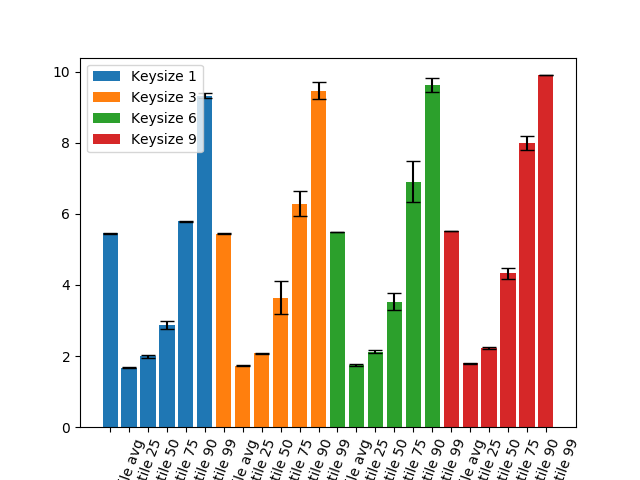
\includegraphics[width=\textwidth]{img/exp5_1/exp5_1_client_percentile_plots_sharded_True.png}
\caption{Exp3.2: Latency and throughputs as measures by the middlewares}
\label{fig:test}
\end{figure}

The multiegets all have a similar response time.
This is because the middleware does not internally distinguish between sending only a single packet, and multiple packets to the servers, as long as these packets fully fit into the \textit{byteBuffer}.
As my byteBuffer is of size $20 * 1024 * 4$, and a single "full" datapacket for message is of size $ 4096 $, this easily fits into the byteBuffer.
As such, there is no significant slowdown in the response time.
However, because of the higher memory requirements, bigger multi-gets tend to be a bit more unstable (as this requires more operations, and more operations can cause delays).
This can be seen in the graph, where the latency percentiles (especially the 90th percentiles) increase with a higher number of keysizes. \\

To do a sanity check, I include the total latency and throughputs as measured by the clients (because the above histogram was derived from client values).
One can clearly see that the trend presented in the above barchart is supported by the response times measured by the clients.
In additional to that, the inverse law for throughput and latency holds, as the throughput and latency both have an overall almost constant tendency (with the exception of the keysize "9" decreasing throughput slightly, and increasing the latency slightly).

\begin{figure}[H]
\centering
\begin{subfigure}{.5\textwidth}
    \centering
    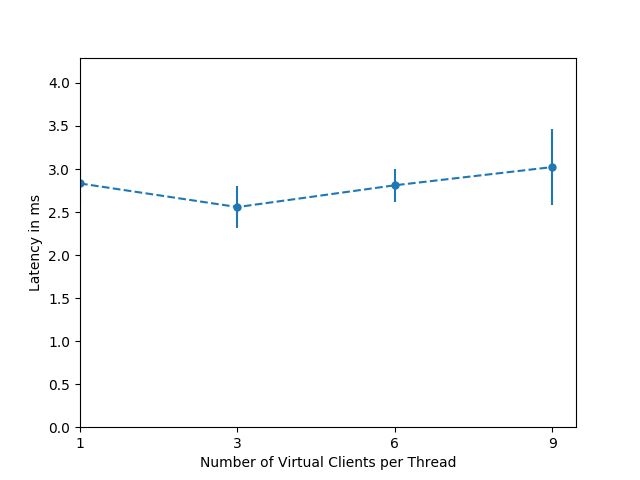
\includegraphics[width=\textwidth]{img/exp5_1/exp5_1__client_latency_sharding_True.png}
    \caption{Latency write only}
    \label{fig:mesh1}
\end{subfigure}%
\begin{subfigure}{.5\textwidth}
      \centering
    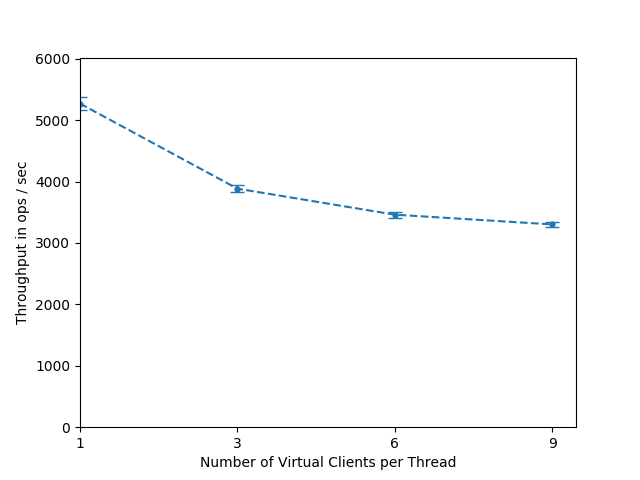
\includegraphics[width=\textwidth]{img/exp5_1/exp5_1__client_throughput_sharding_True.png}
    \caption{Throughput write only}
    \label{fig:mesh1}
\end{subfigure}
\caption{Exp3.2: Latency and throughputs as measures by the clients}
\label{fig:test}
\end{figure}


As a sanity check, the interactive applies, which means that the latency increases when the throughput decreases.
As one can see, the graphs support this claim of the inverse correlation between response time and throughput.

\subsubsection{Explanation}

The bottleneck is either the server which has to respond to all the get-requests (and can do some compoundedly in the case of multi-gets with keysize > 1), or the middleware which does not allow the client to push more requests towards the server.
However, because the bandwidth of the middleware is so high, and theoretically supports almost $35'000 ops/sec$, it is highly likely that it is again the servers which cannot utilize more than the existing bandwidth of $3'000 ops/sec$.
This relates to experiment 2.2 (baseline no middleware, read-only), where one single client instance is able to max out the servers fairly quickly. 
The latency caused by contacting multiple servers instead of just one can be seen by comparing these values to the non-sharded case.
However, this network overhead is negligible as can be seen by comparing the graphs for the sharded case, vs. for the non-sharded case.
\\

However, it could also be the middleware which is not able to pass on all requests quick enough.
This would also explain the drop from $ 6'000 ops/sec $ in experiment 2.2, to $ 3'500 ops/sec$ in this experiment.
After doing a profiling of the code, I recognize that the java function \textbf{String.split} takes up most of the performance, and heavily increases system utilization.

%TODO  average queue length over time! system saturation?

\subsection{Non-sharded Case}

I run multi-gets with 1, 3, 6 and 9 keys (memtier configuration) with sharding disabled. 
The following provides a more detailed view of the configuration that I used.

\begin{center}
	\scriptsize{
		\begin{tabular}{|l|c|}
			\hline Number of servers                & 3                       \\ 
			\hline Number of client machines        & 3                       \\ 
			\hline Instances of memtier per machine & 2                       \\ 
			\hline Threads per memtier instance     & 1                       \\
			\hline Virtual clients per thread       & 2                		 \\ 
			\hline Workload                         & ratio=1:$<$Multi-Get size$>$              \\
			\hline Multi-Get behavior               & Non-Sharded             \\
			\hline Multi-Get size                   & [1..9]                  \\
			\hline Number of middlewares            & 2                       \\
			\hline Worker threads per middleware    & max. throughput config. \\
			\hline Repetitions                      & 3 or more (at least 1 minute each)               \\ 
			\hline 
		\end{tabular}
	} 
\end{center}

I plot average response time as measured on the client, as well as the 25th, 50th, 75th, 90th and 99th percentiles.

\begin{figure}[H]
\centering
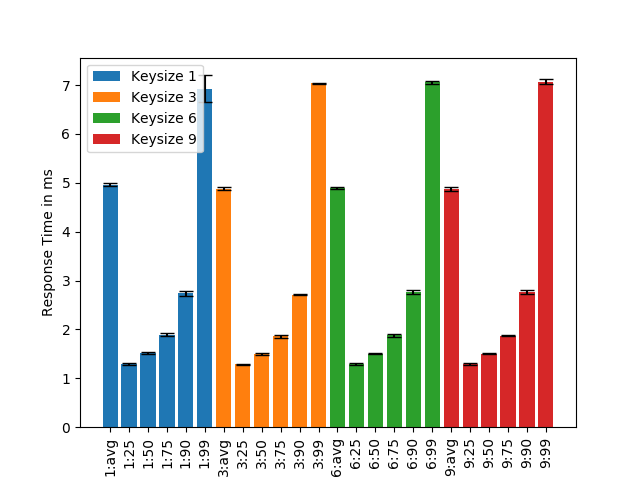
\includegraphics[width=\textwidth]{img/exp5_1/exp5_1_client_percentile_plots_sharded_False.png}
\caption{Exp3.2: Latency and throughputs as measures by the middlewares}
\label{fig:test}
\end{figure}

Internally and inside the middleware, the non-sharded multiegets are treated exactly like multigets with keysize 1.
This means - if the middleware operates well - that the response time and throughput should be very similar for any of the presented multiget keysize values.
And this is indeed the case. 
The average and percentiles match up in response time as can be seen from the graph.
There are some deviations, but these deviations are all within the error bounds of the other multikey-get sizes.
The reason behind the very similar multi-key-getsizes is also the \textit{byteBuffer} that I use, which allows each multikey-get request to fit into the buffer.
As my byteBuffer is of size $20 * 1024 * 4$, and a single "full" datapacket for message is of size $ 4096 $, this easily fits into the byteBuffer.
As such, there is no statistically significant decrease or increase in the response time or throughput. \\

To do a sanity check, I include the total latency and throughputs as measured by the clients (because the above histogram was derived from client values).
One can clearly see that the trend presented in the above barchart is supported by the response times measured by the clients.
In additional to that, the inverse law for throughput and latency holds, as the throughput and latency both have an overall almost constant tendency (with the exception of the keysize "9" decreasing throughput slightly, and increasing the latency slightly).

To double-check that the above graph is correct (mainly the averages of the individual keysizes), I analyse the response time and throughput graphs.
I will only include graphs from the middleware as these values don't include the warm-up and the cool-down times.
However, the values measured as per client do conform with the trends found in the graph. 

\begin{figure}[H]
\centering
\begin{subfigure}{.5\textwidth}
    \centering
    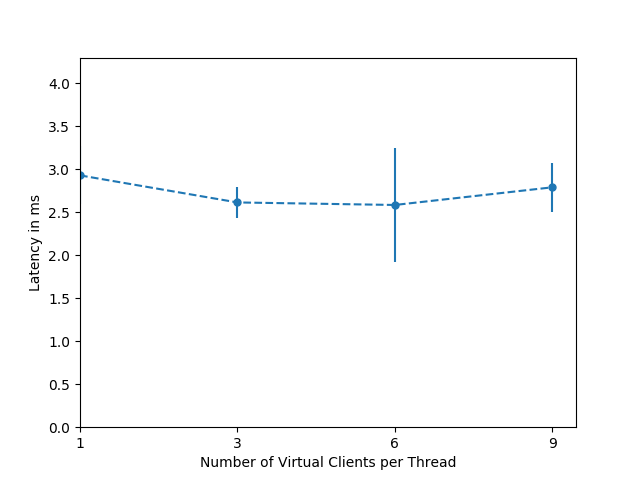
\includegraphics[width=\textwidth]{img/exp5_1/exp5_1__client_latency_sharding_False.png}
    \caption{Latency write only}
    \label{fig:mesh1}
\end{subfigure}%
\begin{subfigure}{.5\textwidth}
      \centering
    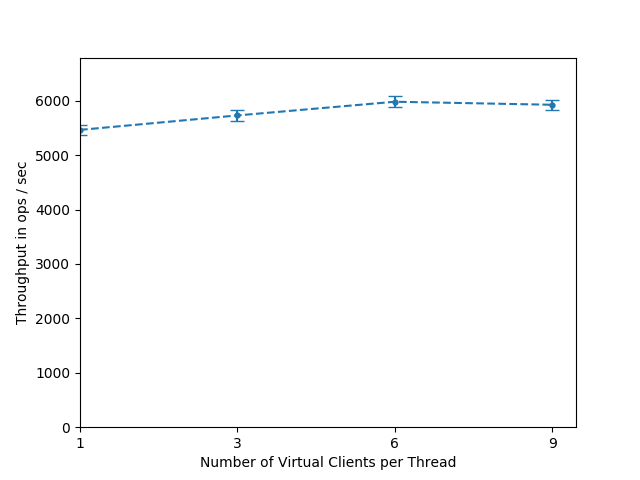
\includegraphics[width=\textwidth]{img/exp5_1/exp5_1__client_throughput_sharding_False.png}
    \caption{Throughput write only}
    \label{fig:mesh1}
\end{subfigure}
\caption{Exp3.2: Latency and throughputs as measures by the clients}
\label{fig:test}
\end{figure}

As a sanity check, the interactive applies, which means that the latency increases when the throughput decreases.
As one can see, the graphs support this claim of the inverse correlation between response time and throughput.

%TODO  average queue length over time! system saturation?
%TODO  code profiling?

\subsubsection{Explanation}

Provide a detailed analysis of the results (e.g., bottleneck analysis, component utilizations, average queue lengths, system saturation). Add any additional figures and experiments that help you illustrate your point and support your claims.

\subsection{Histogram}

For the case with 6 keys inside the multi-get, I now display four histograms representing the sharded and non-sharded response time distribution, both as measured on the client, and inside the middleware. 
I chose the bucket sizes such that the represent intervals of at least 100 micro-seconds (i.e. 1/10th of a millisecond).
After considering taking the mean of multiple items, I arrived at the conclusion of only picking a single memtier-instance's output and plotting this. 
This is for two reasons. 
1. This gives us a more true distribution, and not a flattened mean. Furthermore this is a good approximation, because all latency-histograms (across all memtier-instances) are very similarly distributed.
2. Adding multiple histograms together which are slightly deviated on the x-axis will increase the common latencies (around 2 milliseconds), and proportionally decrease the flatter regions, which also provide information to the reader.
By just picking one instance, I solve this problem and allow for a clearer display of these flat regions (also because the spikes are clearly visible in either case).

\begin{figure}[H]
\centering
\begin{subfigure}{.5\textwidth}
    \centering
    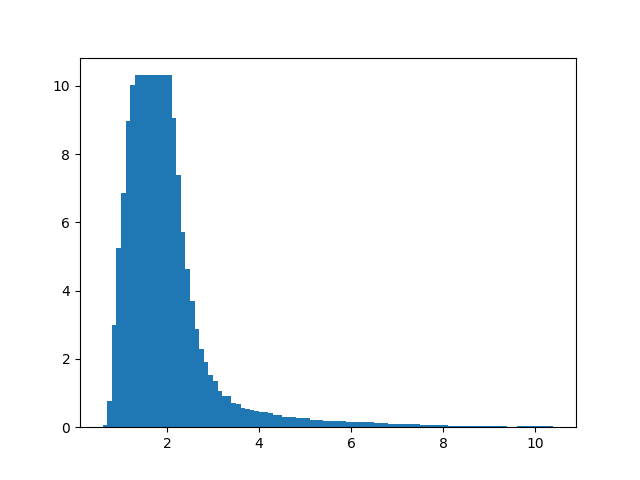
\includegraphics[width=\textwidth]{img/exp5_1/histogram_client_nonsharded.png}
    \caption{Non-Sharded Latency Histogram}
    \label{fig:mesh1}
\end{subfigure}%
\begin{subfigure}{.5\textwidth}
      \centering
    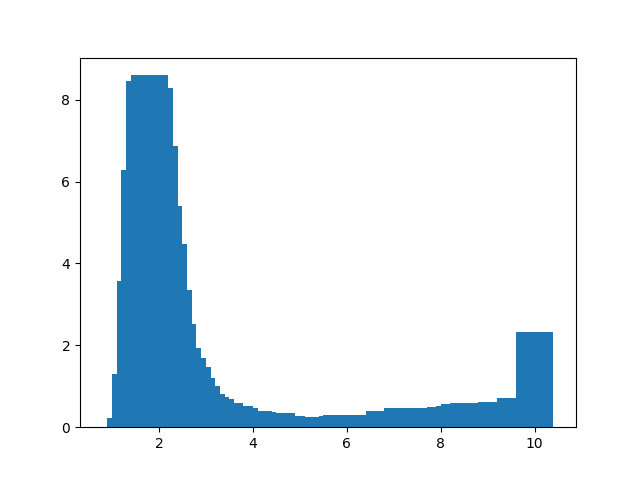
\includegraphics[width=\textwidth]{img/exp5_1/histogram_client_sharded.png}
    \caption{Sharded Latency Histogram}
    \label{fig:mesh1}
\end{subfigure}
\caption{Exp3.2: Latency and throughputs as measures by the clients}
\label{fig:test}
\end{figure}

%TODO fix displaying the 

More network operations come from the fact that more individual servers need to be contact to finish a request (instead of one server, all servers need to be communicated with).
This can be seen in the histogram because the sharded case has a longer tail, as this requires 1. more operations (i.e. more computation effort), as was measured using the tool dstat, and 2. requires more network operations. \\

The client includes the network round-trip between sending it off from the client machine, and arriving at the middleware.
In contrast, the middleware only views latency as the round-trip time from incoming request (right before entering the queue), and right before sending the response back to the client.
This can be seen in the graphs, as the middleware histograms are shifter to the left w.r.t. the client histograms.


\subsection{Summary}

Provide a detailed comparison of the sharded and non-shareded modes. For which multi-GET size is sharding the preferred option? Provide a detailed analysis of your system. Add any additional figures and experiments that help you illustrate your point and support your claims.

\section{2K Analysis (90 pts)}

This 2k analysis includes the analysis of any correlations between the following factors: 1. number of memcached servers, 2. the number of middleware vm's and finally 3. the number of worker threads per middleware.
The following table shows which possible values we cross-reference, such that we can later on analyse which factors have the most impact on throughput and response time.

\begin{itemize}
		
	\item Memcached servers: 1 and 3
	\item Middlewares: 1 and 2
	\item Worker threads per MW: 8 and 32
	      	      
\end{itemize}


Any configuration is run 3 times (3 repetitions) for 90 seconds, which implies a 15 second warm-up and a 15 second cool-down time.
The following table shows a detailed configuration of my setup.

\begin{center}
	\scriptsize{
		\begin{tabular}{|l|c|}
			\hline Number of servers                & 1 and 3                                     \\ 
			\hline Number of client machines        & 3                                           \\ 
			\hline Instances of memtier per machine & 1 (1 middleware) or 2 (2 middlewares) \\ 
			\hline Threads per memtier instance     & 2 (1 middleware) or 1 (2 middlewares)   \\
			\hline Virtual clients per thread       &  32                                     \\ 
			\hline Workload                         & Write-only and Read-only\\
			\hline Number of middlewares            & 1 and 2                                     \\
			\hline Worker threads per middleware    & 8 and 32                                    \\
			\hline Repetitions                      & 3 or more (at least 1 minute each)                                   \\ 
			\hline 
		\end{tabular}
	} 
\end{center}

I apply this analysis once for read-only workloads, and then separately for write-only workloads, as both procedures are fundamentally different.
I don't use any multi-get behavior (i.e. keysize is always 1 for read-only workloads). \\

For read-only and work-only workloads, I created tables which represent all possible configurations.
For both subsections, I will use the following abbreviations (and variable-names)

\begin{itemize}
\item NS: Number of Servers
\item NM: Number of Middlewares
\item WTMW: Worker threads per middleware
\end{itemize}

\subsubsection{Read-only}

% & Mean Latency 

\begin{center}
    \begin{tabular}{ | l | l | l | p{5cm} |}
    \hline
    NS (Servers) & NM (Middlewares) & WTMW (Workerthreads) & Mean Throughput \\ \hline
    1 & 1 & 8 & \\ \hline
    1& 1 & 32 & \\ \hline
    1 & 2 & 8 &  \\ \hline
   	1 & 2 & 32 & \\ \hline
    3 & 1 & 8 & \\ \hline
    3 & 1 & 32 &  \\ \hline
    3 & 2 & 8 &  \\ \hline
    3 & 2 & 32 &  \\
    \hline
    \end{tabular}
\end{center}

Repeat the experiment for (a)~a write-only and (b)~a read-only workload.
For each of the two workloads, what is the impact of these parameters on throughput, respectively response time?




\subsubsection{Write-only}



\section{Queuing Model (90 pts)}

In this section I model the workerqueue of the middleware (after the requests come in) using queueing theory to model how the system behaves with an asymptotically increasing number of threads.
In both subsection I will go use the different number of middleware (specifically, one of [8, 16, 32, 64]) threads to apply this analysis.

\subsection{M/M/1}
In this subsection I model the behavior of the middleware and it's workerqueue using a M/M/1 queueing model. \\

I choose the following input parameters to model the system:

First of all, I define the service rate to the model. 
For this, I look at the maximum throughput per number of middleware threads (amongst all given number of virtual clients). \\
From the file \textbf{create\_lineplot\_exp4\_1.py} I read out the respective maximum throughput values: \\

\begin{center}
	\scriptsize{
		\begin{tabular}{|l|c|}
			\hline Threads in the middleware & Maximum Throughput (ops/sec)                                     \\ 
			\hline 8 &   14365.88 \\ 
			\hline 16 &  18338.97 \\ 
			\hline 32 &  18828.88 \\
			\hline 64 &  17984.48 \\
			\hline
		\end{tabular}
	} 
\end{center}


your entire system. Motivate your choice of input parameters to the model. Explain for which experiments the predictions of the model match and for which they do not.

\subsection{M/M/m}

Build an M/M/m model based on Section 4, where each middleware worker thread is represented as one service.  Motivate your choice of input parameters to the model. Explain for which experiments the predictions of the model match and for which they do not.

\subsection{Network of Queues}

Based on Section 3, build a network of queues which simulates your system. Motivate the design of your network of queues and relate it wherever possible to a component of your system. Motivate your choice of input parameters for the different queues inside the network. Perform a detailed analysis of the utilization of each component and clearly state what the bottleneck of your system is. Explain for which experiments the predictions of the model match and for which they do not.

\section{Appendix}

5.1. throughput and latency as measured by the clients (as opposed to middlewares).
This is the sharded case.

\begin{figure}[H]
\centering
\begin{subfigure}{.5\textwidth}
    \centering
    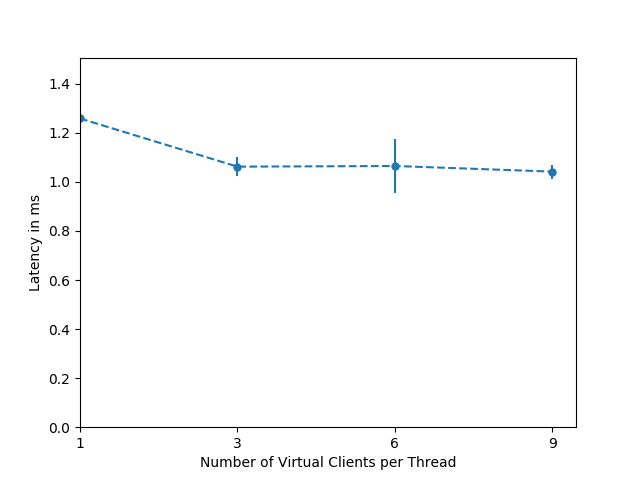
\includegraphics[width=\textwidth]{img/exp5_1/exp5_1__mw_latency_sharding_True.png}
    \caption{Latency write only}
    \label{fig:mesh1}
\end{subfigure}%
\begin{subfigure}{.5\textwidth}
      \centering
    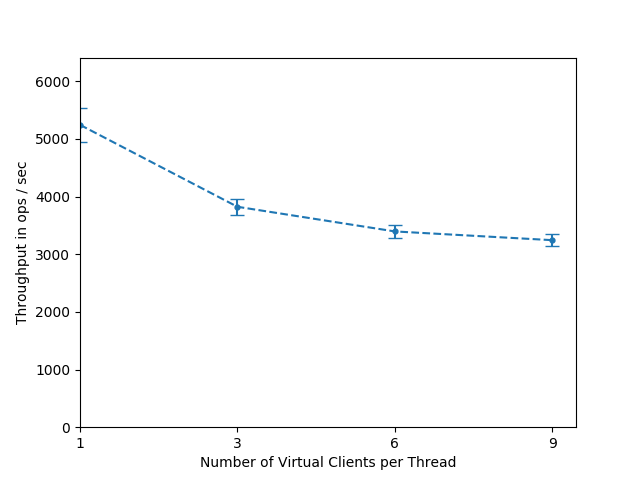
\includegraphics[width=\textwidth]{img/exp5_1/exp5_1__mw_throughput_sharding_True.png}
    \caption{Throughput write only}
    \label{fig:mesh1}
\end{subfigure}
\caption{Exp3.2: Latency and throughputs as measures by the middlewares}
\label{fig:test}
\end{figure}

5.2 throughput and latency as measured by the clients (as opposed to the middlewares).
This is the non-sharded case.

\begin{figure}[H]
\centering
\begin{subfigure}{.5\textwidth}
    \centering
    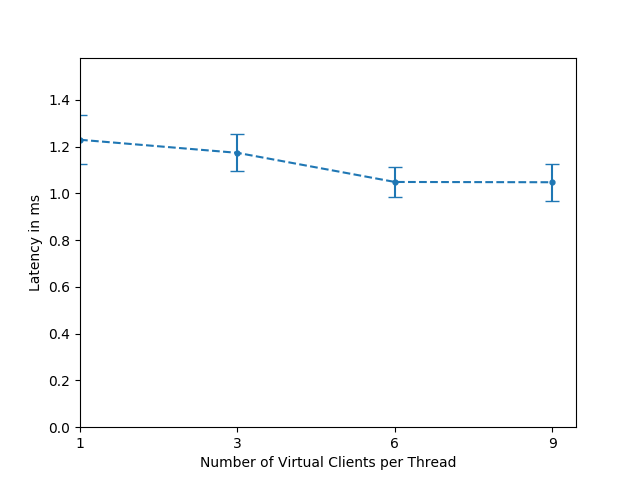
\includegraphics[width=\textwidth]{img/exp5_1/exp5_1__mw_latency_sharding_False.png}
    \caption{Latency write only}
    \label{fig:mesh1}
\end{subfigure}%
\begin{subfigure}{.5\textwidth}
      \centering
    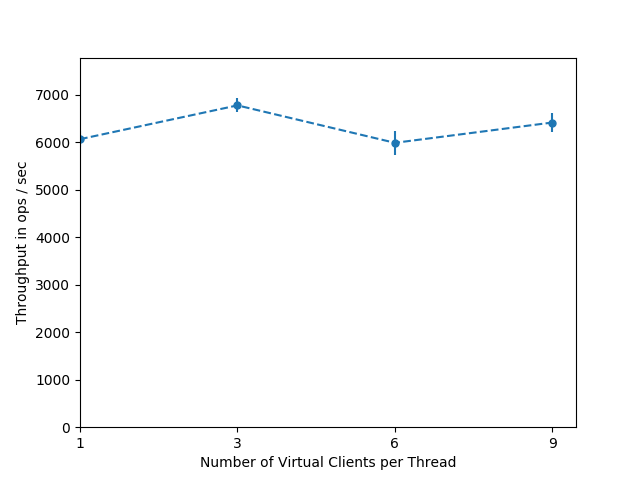
\includegraphics[width=\textwidth]{img/exp5_1/exp5_1__mw_throughput_sharding_False.png}
    \caption{Throughput write only}
    \label{fig:mesh1}
\end{subfigure}
\caption{Exp3.2: Latency and throughputs as measures by the middlewares}
\label{fig:test}
\end{figure}


\end{document}